\documentclass{article}

\PassOptionsToPackage{numbers, compress}{natbib}
\usepackage{neurips_2026}

\usepackage[utf8]{inputenc}
\usepackage[T1]{fontenc}
\usepackage{hyperref}
\usepackage{url}
\usepackage{booktabs}
\usepackage{amsfonts}
\usepackage{amsmath}
\usepackage{amssymb}
\usepackage{amsthm}
\usepackage{nicefrac}
\usepackage{microtype}
\usepackage{xcolor}
\usepackage{graphicx}
\usepackage{multirow}
\usepackage{tikz}
\usetikzlibrary{arrows.meta,decorations.pathreplacing}
\usepackage{enumitem}
\setlist{itemsep=1pt,topsep=3pt,parsep=0pt}

\newtheorem{proposition}{Proposition}
\newtheorem{remark}{Remark}
\newcommand{\R}{\mathbb{R}}
\newcommand{\N}{\mathcal{N}}
\newcommand{\D}{\mathcal{D}}
\newcommand{\NLL}{\mathrm{NLL}}

\input{generated/numbers}

\title{Universal Pool Transformers:\\Robust In-Context Virtual Sensing under Sensor Failure}

\author{Anonymous Authors}

\begin{document}

\maketitle

\begin{abstract}
Virtual sensing predicts the reading of a target sensor from neighbouring sensors. Every deployment is different,
labelled calibration data are scarce, and sensors fail. In-context learners such as TabPFN adapt to a new deployment
from a few labelled rows, but their predictive distributions degrade sharply when input sensors go missing. We
characterize the structure that missing sensors require. Products of per-sensor experts are the free construction on
sensors, the only predictors whose natural parameters are additive over observation masks. Scalar experts cannot
fuse sensors with shared noise, whereas sites \emph{lifted} to a target-plus-nuisance latent are exact for
factor-structured noise. The \emph{Universal Pool Transformer} (UPT) puts a lifted-site head and an unconstrained
head on one transformer backbone and combines them by the linear opinion pool. Its log-likelihood is never worse than
either head's by more than the log of that head's weight, and at initialization it equals the closed-form
factor-analysis posterior up to $0.018$ nats. A scale-free target pipeline removes the fixed scales that limit the
sharpness of the predictive distribution. We evaluate under \NumProtocols{} pre-registered protocols on \NumNetworks{}
real sensor networks in five domains: traffic, indoor climate, air quality, weather and hydrology. \NumFreshNetworks{}
of them were recorded in 2026, after the release of every pretrained model we compare with.
\AbstractResults{}
\end{abstract}

%=====================================================================
\section{Introduction}
%=====================================================================

Sensor networks now measure traffic, air quality, weather and rivers at a density that no maintenance budget can keep
fully operational. \emph{Virtual sensing}, or spatial kriging, predicts a sensor's reading from the readings of its
neighbours. Its uses include filling gaps, standing in for failed or decommissioned instruments, and placing
low-cost virtual sensors where no instrument exists~\citep{wu2021ignnk,cini2022grin}. Three features make the problem
hard.
\begin{enumerate}
  \item \textbf{Deployments differ.} The relation between a target and its neighbours changes from site to site and
  over time, and only a short labelled record is available for each.
  \item \textbf{Noise is shared.} Weather, traffic waves and local emissions move several neighbours at once, so
  neighbours are not conditionally independent given the target.
  \item \textbf{Sensors fail.} At prediction time an arbitrary subset of the neighbours is available, often a subset
  never seen together in the labelled record.
\end{enumerate}

\textbf{In-context virtual sensing.} We cast the problem as in-context probabilistic prediction. A model receives a
deployment's labelled rows (the support), with their missing entries, and a query made of an arbitrary subset of
neighbour readings. It returns a predictive distribution for the target. Trained once, such a model adapts to a new
deployment from its support alone, as neural processes~\citep{garnelo2018cnp,nguyen2022tnp} and prior-fitted networks
do~\citep{muller2022pfn,hollmann2025tabpfnv2}. The pretrained TabPFN v2~\citep{hollmann2025tabpfnv2} is a strong
example. As we show, however, its predictive distribution degrades rapidly as input sensors go missing
(\S\ref{sec:results}).

\textbf{Structure first.} Missing sensors call for a predictor that is defined for every subset of inputs and handles
unseen subsets gracefully.
\begin{itemize}
  \item \textbf{The free construction.} Products of per-sensor experts meet this requirement by construction: a
  missing sensor contributes no factor~\citep{hinton2002poe,wu2018mvae}. We show that this is a universal property,
  not a design choice. Natural-parameter additivity over masks characterizes products of sites, the free
  construction on sensors (Proposition~\ref{prop:free}).
  \item \textbf{Scalar experts are not enough.} With shared noise, no product of mask-independent experts over the
  target alone is Bayes-consistent (Proposition~\ref{prop:scalar}). Sites \emph{lifted} to a latent over target and
  shared nuisance are exact, and need as many nuisance dimensions as the rank of the shared noise
  (Propositions~\ref{prop:exact}--\ref{prop:rank}).
  \item \textbf{Combining with a flexible model.} Real sensors are nonlinear, which favours unconstrained
  transformers. Which rule should combine the structured predictor with a flexible one? The linear opinion pool is
  the rule that commutes with marginalization~\citep{mcconway1981marginalization}. Its log-likelihood is bounded by
  each component's (Proposition~\ref{prop:pool}).
\end{itemize}

\textbf{Contributions.}
\begin{enumerate}
  \item \textbf{Theory (\S\ref{sec:theory}).} Products of sites are the free construction on sensors. Scalar
  experts fail under shared noise, while lifted sites are exact and minimal. The linear pool gives a per-query
  log-likelihood guarantee relative to each component.
  \item \textbf{The Universal Pool Transformer (\S\ref{sec:upt}).} One transformer backbone over the cells of the
  support and the query feeds a lifted-site head, a free head and a gate, combined by the linear pool. At
  initialization UPT is the closed-form factor-analysis (FA) posterior up to $0.018$ nats. A scale-free target
  pipeline makes the predictive equivariant to affine changes of the target's units.
  \item \textbf{A pre-registered evaluation (\S\ref{sec:experiments}).}
  \begin{itemize}
    \item \textbf{Scale:} \NumProtocols{} protocols, each committed before its data were scored, on \NumNetworks{}
    networks and \NumEpisodes{} test episodes.
    \item \textbf{Baselines:} TabPFN v2, a matched-scale transformer, TNP-D, CNP, deep and classical kriging,
    gradient boosting and multiple imputation.
    \item \textbf{Reporting:} every endpoint is reported, including the failures.
  \end{itemize}
\end{enumerate}
\IntroResults{}

%=====================================================================
\section{Problem setup}
\label{sec:setup}
%=====================================================================

\paragraph{Episodes.} An episode concerns one target sensor and its $P$ input sensors in one time window.
\begin{itemize}
  \item The support $\D=\{(x_i,m_i,y_i)\}_{i=1}^{n}$ holds $n=48$ labelled rows. Reading $x_{ij}$ is observed where
  $m_{ij}=1$.
  \item A query is the reading $x_S$ of an observed subset $S\subseteq\{1,\dots,P\}$.
  \item The model returns a predictive density $q(y\mid x_S,\D)$.
\end{itemize}

\paragraph{Scoring.} Methods are scored by the negative log-likelihood (NLL) of held-out targets, the strictly proper
logarithmic score~\citep{gneiting2007scoring}. We also report the CRPS, the RMSE of the predictive mean, and the
coverage of the central 90\% interval.

\paragraph{Training and evaluation splits.} Every learned model is trained on synthetic tasks, then fine-tuned on episodes
from the network's \emph{source} period with an identical recipe for every model. It is evaluated on fixed episodes
from a later \emph{test} period.

\paragraph{Sensor-loss conditions.} In the condition ``$+k$ dropped'', $k$ further observed inputs are removed from each query
at random, on top of the natural missingness.

%=====================================================================
\section{Theory: what missing sensors require}
\label{sec:theory}
%=====================================================================

Write a Gaussian factor over a latent $z\in\R^{L}$ in natural parameters $(\Lambda,\eta)$, where multiplying factors
adds natural parameters. These pairs form a commutative monoid $G$. A site assignment $s:\{1,\dots,P\}\to G$ gives one
factor per sensor. A mask $m\in\{0,1\}^P$ lies in the free commutative monoid $\mathbb{N}^P$.

\begin{proposition}[Products of sites are the free construction]\label{prop:free}
For every site assignment $s$ there is exactly one monoid homomorphism $F:\mathbb{N}^P\to G$ with $F(e_j)=s(j)$,
namely $F(m)=\sum_j m_j s(j)$. Conversely, a predictor whose posterior natural parameters satisfy
$F(A\sqcup B)=F(A)+F(B)-F(\emptyset)$ for disjoint masks is a product of the prior and per-sensor sites.
\end{proposition}

\paragraph{Consequences.} This is the universal property of the free commutative monoid~\citep{maclane1998categories}.
\begin{itemize}
  \item \textbf{Unseen masks.} Every mask, including masks never seen in training, follows from the $P$ sites.
  \item \textbf{New sensors.} A new sensor extends $F$ uniquely.
  \item \textbf{Limitation.} Cross-sensor interactions can enter only through the latent dimension, the Gaussian analogue of
  the limits of sum decompositions~\citep{wagstaff2022universal}.
\end{itemize}

The next two results say how large that latent must be.

\begin{proposition}[Scalar experts]\label{prop:scalar}
Let $x_j=a_jy+d_ju+\sigma_j\epsilon_j$ with independent standard normal $y,u,\epsilon_j$, $\sigma_j>0$ and
$a_j\neq0$. Suppose each expert $t_j(y;x_j)$ is Gaussian in $y$ and does not depend on $S$, and that
$q(y\mid x_S)\propto p(y)\prod_{j\in S}t_j$ is Bayes for all singleton queries. Then $q$ is Bayes for the pair
$\{j,k\}$ if and only if $d_jd_k=0$, and its weight on $x_j$ can have the wrong sign.
\end{proposition}

\paragraph{Lifted sites.} Let $z=(y,h)\in\R^{1+K}$ with $h\sim\N(0,I)$. A lifted site is the rank-one factor of a
linear-Gaussian measurement $x_j=w_j^\top z+c_j+e_j$, with $e_j\sim\N(0,\psi_j)$:
\begin{equation}
  \Lambda_j=\frac{w_jw_j^\top}{\psi_j},\qquad \eta_j=\frac{w_j(x_j-c_j)}{\psi_j},\qquad
  q(z\mid x_S)=\N\!\Big(z;\Lambda^{-1}\eta,\Lambda^{-1}\Big),\quad
  (\Lambda,\eta)=(\Lambda_0,\eta_0)+\textstyle\sum_{j\in S}(\Lambda_j,\eta_j).
  \label{eq:site}
\end{equation}

\begin{proposition}[Exactness and minimal lifting]\label{prop:exact}\label{prop:rank}
If the sensors follow a $K$-factor model with independent errors, \eqref{eq:site} equals $p(z\mid x_S)$ for every $S$.
Conversely, under a generic-rank condition, which holds for almost every loading matrix when $P\geq2K+3$, static
sites over $(y,h)$ with $h\in\R^{K'}$ reproduce $p(y\mid x_S)$ for all $|S|\leq2$ only if $K'\geq K$.
\end{proposition}

\paragraph{Closed-form anchor.} Fitting the factor model to the support by EM with missing
entries~\citep{dempster1977em,rubin1982em} gives a closed-form, mask-exact predictor, which we call
\emph{FA-Gaussian}. Proofs are in Appendix~\ref{app:proofs}.

\paragraph{Pooling with a flexible model.} Real sensors are nonlinear and real noise is not exactly factor-structured, so a
flexible model fits better. To combine the two, we use the linear opinion pool
$p=\pi\,p_{\mathrm{site}}+(1-\pi)\,p_{\mathrm{free}}$. It is the pooling rule that commutes with marginalization
(McConway, 1981)~\citep{mcconway1981marginalization}: pooling joint predictives over $z$ and then marginalizing the
nuisance $h$ gives the same result as marginalizing first. The logarithmic pool is instead the rule that commutes
with Bayesian updating~\citep{genest1984characterization}. We tested it in protocol v5 and report it as an ablation.

\begin{proposition}[Pool guarantee]\label{prop:pool}
For every query and outcome $y$,
\[\NLL_{\mathrm{pool}}(y)\leq\min\{\NLL_{\mathrm{site}}(y)-\log\pi,\ \NLL_{\mathrm{free}}(y)-\log(1-\pi)\}.\]
In particular, when the free component fails under sensor loss, the pool loses at most $-\log\pi$ relative to the
lifted site, which handles any mask exactly.
\end{proposition}

%=====================================================================
\section{The Universal Pool Transformer}
\label{sec:upt}
%=====================================================================

\begin{figure}[t]
\centering
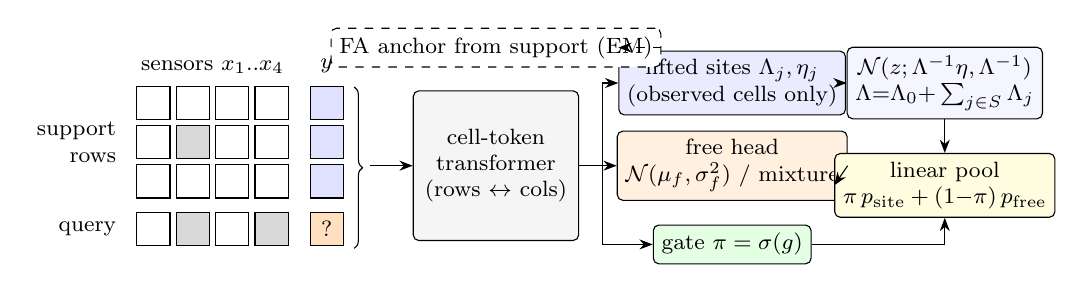
\begin{tikzpicture}[
  font=\footnotesize, >=Stealth,
  box/.style={draw, rounded corners=2pt, align=center, inner sep=3pt},
  tok/.style={draw, minimum width=4.2mm, minimum height=4.2mm, inner sep=0pt},
]
% cell grid: support rows (3 shown) and one query row; columns x1..x4 and target y
\foreach \r/\lab in {0/{support}, 1/{}, 2/{}} {
  \foreach \c in {0,...,3} { \node[tok] at (\c*0.5, -\r*0.5) {}; }
  \node[tok, fill=blue!12] at (2.2, -\r*0.5) {};
}
\node[tok, fill=black!15] at (0.5, -0.5) {};
\node[tok] at (0, -1.6) {}; \node[tok, fill=black!15] at (0.5, -1.6) {}; \node[tok] at (1.0, -1.6) {}; \node[tok, fill=black!15] at (1.5, -1.6) {};
\node[tok, fill=orange!25] at (2.2, -1.6) {?};
\node[left, align=right] at (-0.35, -0.5) {support\\rows};
\node[left] at (-0.35, -1.6) {query};
\node[above] at (0.75, 0.25) {sensors $x_1..x_4$};
\node[above] at (2.2, 0.25) {$y$};
\draw[decorate, decoration={brace, amplitude=3pt}] (2.55, 0.2) -- (2.55, -1.85);
% backbone
\node[box, minimum width=2.1cm, minimum height=1.9cm, fill=gray!8] (bb) at (4.35, -0.8) {cell-token\\transformer\\(rows $\leftrightarrow$ cols)};
\draw[->] (2.75, -0.8) -- (bb.west);
% heads
\node[box, fill=blue!8] (site) at (7.35, 0.25) {lifted sites $\Lambda_j,\eta_j$\\(observed cells only)};
\node[box, fill=orange!12] (free) at (7.35, -0.8) {free head\\$\N(\mu_f,\sigma_f^2)$ / mixture};
\node[box, fill=green!10] (gate) at (7.35, -1.8) {gate $\pi=\sigma(g)$};
\draw[->] (bb.east) -- ++(0.3,0) |- (site.west);
\draw[->] (bb.east) -- (free.west);
\draw[->] (bb.east) -- ++(0.3,0) |- (gate.west);
\node[box, fill=blue!4] (post) at (10.05, 0.25) {$\N(z;\Lambda^{-1}\eta,\Lambda^{-1})$\\$\Lambda{=}\Lambda_0{+}\sum_{j\in S}\Lambda_j$};
\draw[->] (site) -- (post);
\node[box, fill=yellow!12] (pool) at (10.05, -1.05) {linear pool\\$\pi\,p_{\mathrm{site}}+(1{-}\pi)\,p_{\mathrm{free}}$};
\draw[->] (post) -- (pool);
\draw[->] (free.east) -- (pool.west);
\draw[->] (gate.east) -| (pool.south);
\node[box, dashed, fill=white] (fa) at (4.35, 0.7) {FA anchor from support (EM)};
\draw[->, dashed] (fa.east) -- (site.west |- fa.east) ;
\end{tikzpicture}
\caption{\textbf{The Universal Pool Transformer.} One transformer reads every cell of the support and the query
(grey: missing). The query's observed cells emit corrections to their factor-analysis anchor sites, which combine
exactly by adding natural parameters, so a missing sensor simply contributes nothing. The target token emits an
unconstrained predictive and a gate, and the output is their linear opinion pool. With a zero site head the model is
the closed-form FA posterior (Proposition~\ref{prop:init}).}
\label{fig:method}
\end{figure}


\paragraph{Backbone.} UPT uses a cell-token transformer over the support and the queries, in the style of
TabPFN~\citep{hollmann2025tabpfnv2}.
\begin{itemize}
  \item \textbf{Tokens.} Every cell (row $i$, column $j$) becomes a token: the embedded value, or a learned \emph{missing}
  embedding, plus a random feature embedding that distinguishes the columns.
  \item \textbf{Target column.} It carries the standardized support targets, and a learned query embedding in the query rows.
  \item \textbf{Attention.} Blocks alternate attention across the columns of a row and across the rows of a column. Query rows
  attend only to support rows.
\end{itemize}

\paragraph{Three heads on the query tokens.}
\begin{enumerate}
  \item \textbf{Lifted-site head.} Each observed query cell $j$ outputs a correction
  $(\delta^{\mathrm{off}}_j,\delta^{\mathrm{slope}}_j,\delta^{D}_j,s_j)$ to its FA anchor site. The corrected site is
  the local linearization of sensor $j$'s response at the anchor's prediction, and the sites combine by
  \eqref{eq:site}. Missing cells contribute nothing.
  \item \textbf{Free head.} The target-column token outputs a Gaussian, or a small Gaussian mixture.
  \item \textbf{Gate.} The same token outputs $\pi=\sigma(g)$. The predictive is the linear pool
  $\pi\,p_{\mathrm{site}}+(1-\pi)\,p_{\mathrm{free}}$.
\end{enumerate}

\paragraph{Cost.} The heads add $3d+3$ parameters (about 0.1\%), and inference is one backbone pass.

\begin{proposition}[Initialization]\label{prop:init}
With a zero site head and gate bias $+4$, the lifted site equals the FA-Gaussian, so for every query and outcome
$\NLL_{\mathrm{UPT}}\leq\NLL_{\mathrm{FA}}-\log\sigma(4)=\NLL_{\mathrm{FA}}+0.018$.
\end{proposition}

\paragraph{Scale-free target pipeline (SF).} In-context transformers standardize the target internally. Our backbone
inherited two fixed scales from its synthetic prior:
\begin{itemize}
  \item a floor of $0.1$ on the support standard deviation;
  \item a bound of $\pm5$ on the output log-variance.
\end{itemize}

The FA anchor also carries absolute ridges. On targets that vary little within an episode, these floors cap how sharp
the predictive can be (\S\ref{sec:results}). SF removes them:
\begin{itemize}
  \item each episode's target is standardized by its support mean and standard deviation before the anchor fit and the
  network;
  \item the log-variance bound is widened to $\pm10$;
  \item predictions are mapped back to raw units ($\NLL+\log s$).
\end{itemize}

Because the inputs are already standardized per episode, the whole predictive becomes equivariant to affine changes
of the target's units. We check this exactly in our test suite.

\paragraph{Training.} We pretrain on synthetic factor-model tasks with nonlinear sensor responses. Query masks remove at most
one sensor. Then we fine-tune on source-period episodes of each network.
\begin{itemize}
  \item \textbf{Pretraining:} 30k steps for small models and 40k for large ones.
  \item \textbf{Fine-tuning:} 2{,}000 steps, with one recipe for every model.
  \item \textbf{UPT-L:} 2.1M parameters ($d=128$, 8 layers).
  \item \textbf{Objective:} NLL, optionally plus the closed-form mixture CRPS~\citep{grimit2006crps}, a sum of strictly proper
  scores.
  \item \textbf{Prediction:} we average 8 random feature embeddings by an equal-weight linear pool, the analogue of TabPFN's
  8-member ensemble.
\end{itemize}

%=====================================================================
\section{Experiments}
\label{sec:experiments}
%=====================================================================

\paragraph{Pre-registration.} We ran \NumProtocols{} protocols (v5--v13). Each was committed to a public repository
before any score on its test data existed. Each fixes:
\begin{itemize}
  \item networks, splits and seeded test panels;
  \item model recipes;
  \item endpoints, statistics and pass rules.
\end{itemize}
Every endpoint is reported, failures included (Table~\ref{tab:all-endpoints}). Model changes were selected on data
already used by an earlier protocol, by rules written into the next protocol, and then confirmed on networks never
used before (v9, v10).

\paragraph{Networks.} The thirteen networks are listed in Table~\ref{tab:networks}.
\begin{itemize}
  \item \textbf{Traffic:} speed on METR-LA and PEMS-BAY, flow on PeMS03 and PeMS08.
  \item \textbf{Indoor climate:} Intel Lab temperature.
  \item \textbf{Air quality:} PM$_{2.5}$ in China and the UK; NO$_2$ in the UK.
  \item \textbf{Weather:} temperature and pressure from the German weather service.
  \item \textbf{Hydrology:} river discharge from three US states.
\end{itemize}
Seven networks have test periods in April--September 2026, after the release of TabPFN v2 (January 2025).
TabPFN-3.5 was released on September 9, 2026, near the end of these periods. We cannot rule out that its training
data include some of these public records; that would favour TabPFN-3.5, not our models.

\paragraph{Episodes and conditions.} Each test episode predicts one held-out sensor from its 11 neighbours. It has
48 labelled support rows from the same time window, a day to a week. Metrics are computed on 48 query rows, under
three conditions:
\begin{itemize}
  \item the natural mask, ``all sensors'';
  \item $+3$ further inputs dropped at random;
  \item $+6$ further inputs dropped at random.
\end{itemize}

\paragraph{Baselines.}
\begin{itemize}
  \item \textbf{TabPFN v2}~\citep{hollmann2025tabpfnv2}, in context with 8 estimators. Missing inputs are passed as
  NaN.
  \item \textbf{TabPFN-3.5}~\citep{jaeger2026tabpfn35}, the default model of the \texttt{tabpfn} package since
  September 2026, run exactly like TabPFN v2 (8 estimators, its default) on the four 2026 networks (protocol v13).
  \item \textbf{PFN-L.} A plain cell-token transformer with UPT's backbone, size and training budget, but only the
  free head: the matched-scale ablation. It is trained with the same SF pipeline and test-time ensemble as UPT.
  \item \textbf{Neural processes:} TNP-D~\citep{nguyen2022tnp} and CNP~\citep{garnelo2018cnp}, trained on the same
  prior and fine-tuned with the same recipe.
  \item \textbf{Deep kriging:} an IGNNK-style inductive kriging model~\citep{wu2021ignnk} trained on each network's
  source period. Its \emph{calibrated} variant is recalibrated by an affine map on each episode's support, the
  stronger of the two.
  \item \textbf{Closed forms:} FA-Gaussian (UPT's anchor) and EM-Gaussian (simple kriging).
  \item \textbf{Tabular baselines:} LightGBM and multiple imputation (Appendix~\ref{app:results}).
\end{itemize}
UPT-SF is UPT-L with the SF pipeline, the CRPS-augmented objective and the 8-member test-time ensemble, chosen by the
pre-registered rule of protocol v10.

\subsection{Results}
\label{sec:results}

\begin{table}[t]\centering\small
\caption{\textbf{Pre-registered endpoints on the four fresh 2026 networks.} NLL gain in nats (baseline $-$ ours; positive favours the first method), paired 95\% interval clustered by network-window; \checkmark: pass (gain $\geq 0.01$ and lower bound $>0$). Protocols v12 and v13 (TabPFN-3.5, September 2026) test the mechanism and a newer foundation model on the same networks after v11; v14 tests the variant selected on development networks, and $^\dagger$ marks a secondary comparison.}
\label{tab:fresh}
\setlength{\tabcolsep}{3pt}
\begin{tabular}{llccc}
\toprule
Protocol & Comparison & All inputs & 3 dropped & 6 dropped \\
\midrule
v11 & UPT-SF$\oplus$TabPFN vs TabPFN v2 & +0.17 [+0.14, +0.20] \checkmark & +0.24 [+0.20, +0.29] \checkmark & +0.60 [+0.49, +0.72] \checkmark \\
v11 & UPT-SF$\oplus$TabPFN vs UPT-SF alone & +0.91 [+0.76, +1.06] \checkmark & -- & -- \\
v13 & UPT-SF$\oplus$TabPFN-3.5 vs TabPFN-3.5 & +0.04 [+0.03, +0.06] \checkmark & +0.03 [+0.01, +0.04] \checkmark & +0.03 [+0.01, +0.04] \checkmark \\
v13 & UPT-SF$\oplus$TabPFN-3.5 vs UPT-SF alone & +1.33 [+1.13, +1.53] \checkmark & -- & -- \\
v14 & UPT site$\,\otimes\,$TabPFN-3.5 vs TabPFN-3.5 & +0.01 [-0.01, +0.03] $\times$ & -0.01 [-0.06, +0.04] $\times$ & +0.01 [-0.02, +0.05] $\times$ \\
v14$^\dagger$ & UPT site$\,\otimes\,$TabPFN-3.5 vs UPT-SF$\oplus$TabPFN-3.5 & -0.03 [-0.05, -0.02] $\times$ & -0.04 [-0.08, +0.01] $\times$ & -0.01 [-0.04, +0.02] $\times$ \\
v12 & UPT-SF$\oplus$TabPFN vs PFN-L$\oplus$TabPFN & +0.12 [+0.08, +0.16] \checkmark & +0.12 [+0.08, +0.16] \checkmark & +0.09 [+0.05, +0.12] \checkmark \\
v12 & UPT-SF$\oplus$TabPFN vs FA$\oplus$TabPFN & +0.10 [+0.08, +0.12] \checkmark & +0.11 [+0.10, +0.13] \checkmark & +0.12 [+0.10, +0.13] \checkmark \\
v10 & UPT-SF alone vs TabPFN v2 & -0.75 [-0.93, -0.58] $\times$ & -0.63 [-0.81, -0.45] $\times$ & -0.21 [-0.44, +0.03] $\times$ \\
\bottomrule
\end{tabular}
\end{table}

\begin{figure}[t]
\centering
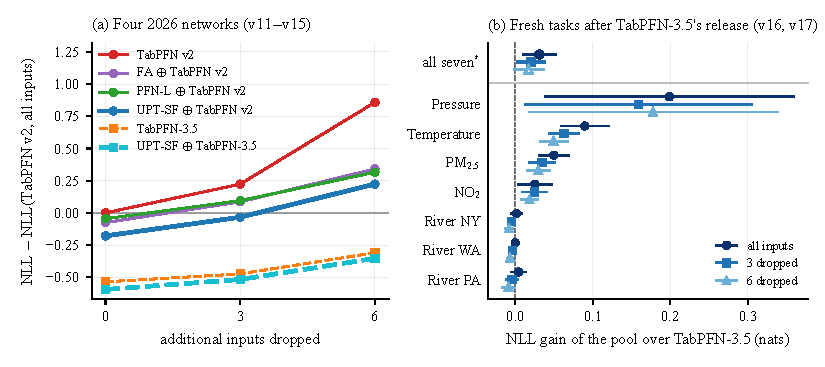
\includegraphics[width=\linewidth]{figures/pool_fresh.pdf}
\caption{\textbf{(a) Robustness to failing inputs} on the four 2026 networks: mean NLL relative to TabPFN v2 with all
inputs. TabPFN v2 degrades by 0.86 nats at six dropped inputs; pooling it with any partner helps, and UPT is the best
partner. TabPFN-3.5 (dashed) is far stronger and more robust; pooling it with UPT (v15 rule) still improves it at every
level. \textbf{(b) Fresh tasks recorded after TabPFN-3.5's release:} NLL gain of the frozen v15 pool over TabPFN-3.5 on
each network (95\% $t$-intervals over network-windows; descriptive) and on all seven pooled ($^*$the pre-registered
endpoints, 97.5\% intervals; open marker: the interval reaches zero).}
\label{fig:robust}
\end{figure}

\paragraph{UPT\,$\oplus$\,TabPFN on fresh 2026 data (protocols v11, v12).} Every pre-registered endpoint of the
pooled model passes (Table~\ref{tab:fresh}, pooled over \FreshEpisodes{} episodes on four networks).
\begin{itemize}
  \item \textbf{Against TabPFN v2,} the gain grows with the number of failed inputs: \XOne{} nats with all inputs,
  \XTwoThree{} with three dropped, \XTwoSix{} with six dropped.
  \item \textbf{On each network separately} the pool beats TabPFN v2 too: by 0.07--0.44 nats with all inputs and by
  0.16--1.69 with six dropped (Table~\ref{tab:pool}).
  \item \textbf{The stacking weights are interpretable.} With no test label, they place 72--83\% of the weight on
  TabPFN for the two river networks with all inputs, whose near-deterministic targets suit its sharp predictive. They place 68--97\%
  on UPT for pressure and PM$_{2.5}$, rising as inputs fail. With TabPFN-3.5 they track the two models' relative skill
  in the same way (Figure~\ref{fig:weights}).
\end{itemize}

\paragraph{Is it the partner or just pooling? (protocol v12).} Pooling TabPFN with any reasonable partner helps under
input failure: TabPFN alone loses 0.86 nats at six dropped inputs (Figure~\ref{fig:robust}a). The partner still
matters. With the same stacking rule, UPT is a better partner than:
\begin{itemize}
  \item the plain transformer of equal size and training: \YOneZero{} nats with all inputs, \YOneSix{} with six
  dropped;
  \item the closed-form lifted sites: \YTwoZero{} and \YTwoSix{}.
\end{itemize}
Both ingredients of UPT therefore contribute: the lifted sites beat the plain transformer, and the learning beats
the closed form. The largest margin is on the pressure network: UPT\,$\oplus$\,TabPFN scores $-0.60$ against $-0.12$
for PFN-L\,$\oplus$\,TabPFN.

\paragraph{The newest foundation model (protocols v13, v15).} TabPFN-3.5 (September 2026) is far stronger than
TabPFN v2 on these networks (by 0.3--1.3 nats) and degrades much less when inputs fail. The same pool, run unchanged
(v13), still improves it: \ZOne{} nats with all inputs, \ZTwoThree{} and \ZTwoSix{} with three and six dropped. On
pressure, UPT alone beats TabPFN-3.5 at every level ($-0.57$ vs $-0.47$ with all inputs), and UPT is a better partner
than a plain transformer by $+0.05$ to $+0.07$ nats. On the rivers, however, the pool lost 0.015--0.03 nats. With learning-curve-aware stacking (v15,
selected on development networks), the gains grow to \VOne{}, \VTwoThree{} and \VTwoSix{} nats, the pool beats the
v13 pool at every level (\VPoolZero{} with all inputs), and the river losses shrink by 75--95\%, to at most 0.008
nats (Figure~\ref{fig:crossfit}). The pre-registered claim that it is never worse than TabPFN-3.5 on any network fails narrowly: \VThreePass{} of
\VThreeN{} non-inferiority tests pass, the three failures being rivers with inputs dropped.

\paragraph{Fresh tests after TabPFN-3.5's release (protocols v16, v17).} The test periods of v13--v15 precede
TabPFN-3.5's release. We therefore froze the v15 rule and scored it once on new tasks: days after the release
(September 10 -- October 12) and 48 target sensors per network that no protocol had used. On the four v10 networks
(v16) the pool beats TabPFN-3.5 with all sensors (\FOne{} nats); with inputs dropped the gains (\FTwoThree{},
\FTwoSix{}) are as large as v15 predicted, but with 30 clusters their intervals reach zero. v17 added the three v9
networks and tested all \GEpisodes{} tasks (\GClusters{} clusters) at the 97.5\% level of a second look: the pool wins
with all sensors (\GOne{}) and with three dropped (\GTwoThree{}); with six dropped (\GTwoSix{}) the interval reaches
zero. Gains are large where UPT alone beats TabPFN-3.5 (pressure, temperature) and smaller on air quality; rivers tie
with all sensors and lose at most 0.009 nats with inputs dropped (Figures~\ref{fig:robust}b and~\ref{fig:fresh-curves}).

\paragraph{Beyond averaging fails confirmation (protocol v14).} A linear pool is never sharper than its sharper member
on a single query. Of the combinations that could be (UPT's predictive as inputs of TabPFN-3.5, TabPFN-3.5 on UPT's
residuals, the logarithmic pool $p\propto p_F^a\,\mathcal N(m_{\mathrm{UPT}},v_{\mathrm{UPT}})^b$), development
selected the logarithmic pool, which then failed every confirmatory endpoint (\ROne{}, \RTwoThree{}, \RTwoSix{}),
losing up to 0.12 nats on rivers: unlike the linear pool (Proposition~\ref{prop:pool}), it has no loss bound.

\begin{table}[t]\centering\small
\caption{\textbf{Mean test NLL (nats; lower is better)} with all sensors (left of the slash) and with six extra sensors dropped (right). Learned models: mean over three seeds. Best per row in bold. Networks recorded in 2026 are below the rule; the last four are protocol v10, never used before its endpoints were scored. On USGS NY the UPT-SF mean is dominated by 15 episodes with a constant support target (\S\ref{sec:results}).}
\label{tab:main}
\setlength{\tabcolsep}{3pt}
\begin{tabular}{lcccccc}
\toprule
Network & UPT-SF & PFN-L & TabPFN v2 & TNP-D & Krig.\ (cal.) & FA-Gauss. \\
\midrule
METR-LA & \textbf{-1.82}/\textbf{-1.60} & -1.48/-1.09 & -1.79/-1.21 & -1.37/-0.44 & -0.50/+0.30 & -0.15/-0.29 \\
PEMS-BAY & \textbf{-2.68}/\textbf{-2.34} & -2.42/-2.03 & -2.68/-2.06 & -2.11/-0.92 & -1.46/-0.57 & -0.94/-1.02 \\
Intel Lab & -0.95/\textbf{-0.02} & -0.32/+0.79 & \textbf{-1.30}/+2.36 & +0.03/+1.75 & +0.94/+2.72 & +0.49/+0.64 \\
PeMS03 & \textbf{-1.30}/\textbf{-1.00} & -1.03/-0.80 & -1.04/-0.04 & -0.93/-0.16 & -0.42/-0.34 & -0.57/-0.52 \\
PeMS08 & \textbf{-2.54}/\textbf{-2.12} & -1.12/-1.01 & -1.82/-0.62 & -1.07/-0.43 & -0.68/-0.94 & -1.28/-1.27 \\
China air & \textbf{-0.25}/\textbf{-0.03} & -0.12/+0.06 & -0.24/+0.92 & -0.05/+0.21 & +0.17/+0.51 & +0.27/+0.26 \\
\midrule
DWD temp. & \textbf{+1.02}/\textbf{+1.22} & +1.04/+1.25 & +1.32/+2.14 & +1.19/+1.62 & +1.39/+1.49 & +1.52/+1.45 \\
AURN NO$_2$ & \textbf{+0.22}/\textbf{+0.41} & +0.23/+0.44 & +0.30/+0.62 & +0.31/+0.55 & +0.37/+0.54 & +0.47/+0.51 \\
USGS PA & -2.62/-2.27 & -2.26/-1.97 & \textbf{-3.66}/\textbf{-2.72} & -1.82/-0.91 & -0.82/-0.37 & -0.86/-1.08 \\
USGS NY & +2024.7/+1305.6 & -1.56/-1.34 & \textbf{-3.63}/\textbf{-2.88} & -1.41/-0.75 & +85.3/+85.8 & -0.17/-0.26 \\
USGS WA & -3.31/-2.98 & -2.73/-2.47 & \textbf{-4.97}/\textbf{-4.41} & -2.51/-2.11 & -1.95/-1.78 & -2.22/-2.24 \\
DWD pressure & \textbf{-0.57}/\textbf{-0.22} & -0.01/+0.14 & -0.15/+1.46 & +0.09/+1.40 & +0.15/+0.65 & +0.07/+0.03 \\
AURN PM$_{2.5}$ & -0.40/\textbf{-0.21} & -0.27/-0.10 & \textbf{-0.43}/+0.07 & -0.21/+0.06 & -0.07/+0.08 & +0.13/+0.08 \\
\bottomrule
\end{tabular}
\end{table}

\paragraph{UPT alone across thirteen networks (protocols v6--v10; Table~\ref{tab:main}).} At matched size and
training, UPT has a lower mean NLL than the plain transformer on 12 of 13 networks at every sensor-loss level. It
beats TNP-D on all six v6/v7 networks (pre-registered v8: $+0.38$, $+0.53$, $+1.05$ nats at 0, 3, 6 dropped) and
calibrated deep kriging by more than one nat. Against TabPFN v2 alone it is better on 10 of 13 networks with six
inputs dropped ($+0.33$ nats pooled, descriptive) and on 8 of 13 with all inputs.

\paragraph{Failures.} We report all of them (Appendix~\ref{app:protocols}).
\begin{enumerate}
  \item \textbf{UPT alone loses to TabPFN v2 on the river networks} (v9, v10). The pre-registered pooled NLL tests of
  UPT alone against TabPFN on the 2026 networks fail. On rivers TabPFN's predictive is far sharper, at about the same
  RMSE; UPT's synthetic prior (five sensors, one factor) is far narrower than TabPFN's.
  \item \textbf{A degenerate case.} When all 48 support targets are identical (15 of 1{,}437 New York episodes),
  UPT's predictive collapses; this breaks v10's comparisons of UPT alone with the transformer, TNP-D and kriging.
  \item \textbf{With all inputs, TabPFN v2 alone remains better on 5 of 13 networks} (v6 P3, v9). Ablations from
  earlier protocols are in Appendix~\ref{app:protocols}.
\end{enumerate}



%=====================================================================
\section{Related work}
\label{sec:related}
%=====================================================================

\paragraph{Kriging and virtual sensing.} Graph neural kriging trains on a network's history and transfers to unseen nodes,
for example IGNNK~\citep{wu2021ignnk}, GRIN~\citep{cini2022grin} and spatio-temporal neural
processes~\citep{hu2023stgnp}. We compare with an IGNNK-style model, recalibrated in context on each episode's
support. In-context models avoid retraining under drift.

\paragraph{Neural processes and prior-fitted networks.} CNP~\citep{garnelo2018cnp}, TNP~\citep{nguyen2022tnp},
PFNs~\citep{muller2022pfn} and TabPFN~v2~\citep{hollmann2025tabpfnv2} learn to predict from a context set. They
handle missing inputs implicitly. UPT adds an explicit structured component that handles missing inputs exactly.

\paragraph{Products of experts and opinion pools.} Products of experts handle missing modalities by
omission~\citep{hinton2002poe,wu2018mvae}. Generalized products~\citep{cao2014gpoe} and power EP~\citep{minka2004power}
temper experts. The axiomatic theory of opinion pools~\citep{mcconway1981marginalization,genest1984characterization}
characterizes the linear and logarithmic pools.

\paragraph{Learned message passing.} Learned EP~\citep{heess2013learning} and unrolled inference~\citep{gregor2010lista}
amortize factor updates. Our lifted sites read their corrections from transformer tokens.

\paragraph{Missing values in supervised learning.} NeuMiss~\citep{lemorvan2020neumiss} unrolls the Bayes predictor of a
Gaussian model, but it is trained per dataset.

%=====================================================================
\section{Limitations}
\label{sec:limits}
%=====================================================================
\begin{itemize}
  \item \textbf{Cost.} UPT\,$\oplus$\,TabPFN runs both models, plus two half-support cross-fit calls per episode for
  the stacking weight.
  \item \textbf{UPT alone vs TabPFN.} On near-deterministic targets (river discharge), UPT alone is markedly less sharp
  than TabPFN v2. Its synthetic prior (five sensors, one factor) is far narrower than TabPFN's.
  \item \textbf{A degenerate case.} UPT's scale-free target standardization breaks down when every support target of
  an episode is identical (15 of 5{,}346 fresh episodes). This was found after the fact; the fix is untested.
  \item \textbf{Baselines.} We compare with TabPFN v2, not its later versions, and with a local-graph adaptation of
  inductive kriging rather than full-graph, temporal models (GRIN~\citep{cini2022grin}, graph neural
  processes~\citep{hu2023stgnp}). Those models may do better when a long, stationary history is available.
  \item \textbf{Episodes.} Episodes treat rows within a window as exchangeable and ignore temporal order.
  \item \textbf{Provisional data.} The 2025--2026 data are provisional and may be revised. We release the snapshots'
  content digests and the code that downloads them.
  \item \textbf{Protocol history.} Protocol v12 tests a mechanism on networks already used by v10 and v11. Its
  endpoints are pre-registered, but the data are not fresh.
\end{itemize}


%=====================================================================
\section{Conclusion}
%=====================================================================
The structure that missing sensors require is unique: products of per-sensor sites, lifted to a target-plus-nuisance
latent, combined with flexible models by the linear opinion pool. The Universal Pool Transformer realizes it in one
network, and the same pool makes pretrained foundation models more robust to sensor failure: under pre-registered
protocols on networks recorded in 2026, UPT\,$\oplus$\,TabPFN improved both TabPFN v2 and the much stronger
TabPFN-3.5, with UPT the best partner. A richer pretraining prior would close the remaining gap of UPT alone on
near-deterministic targets.


\bibliographystyle{plainnat}
\bibliography{references}

\clearpage
\appendix
\section{Proofs}
\label{app:proofs}

\paragraph{Proposition~\ref{prop:free}.}
$\mathbb{N}^P$ is the free commutative monoid on $\{1,\dots,P\}$: every $m$ is uniquely $\sum_j m_je_j$. A homomorphism
$F$ with $F(e_j)=s(j)$ must therefore satisfy $F(m)=\sum_jm_jF(e_j)=\sum_jm_js(j)$, and this formula is a
homomorphism, because addition in $G$ is commutative and associative~\citep{maclane1998categories}.

For the converse, let $F_0=F(\emptyset)$ be the prior's natural parameters and set $s(j)=F(\{j\})-F_0$. If
$F(A\sqcup B)=F(A)+F(B)-F_0$ for all disjoint $A,B$, induction on $|S|$ gives $F(S)=F_0+\sum_{j\in S}s(j)$. The
posterior is thus the prior times one factor per observed sensor. \hfill$\square$

\paragraph{Proposition~\ref{prop:pool}.}
Both mixture components are non-negative. Hence
$p_{\mathrm{pool}}(y)\geq\pi\,p_{\mathrm{site}}(y)$ and $p_{\mathrm{pool}}(y)\geq(1-\pi)\,p_{\mathrm{free}}(y)$.
Taking $-\log$ of each gives the two bounds.

Marginalization commutes with the linear pool by linearity of the integral:
$\int(\pi p_1+(1-\pi)p_2)\,dh=\pi\int p_1\,dh+(1-\pi)\int p_2\,dh$. McConway~\citep{mcconway1981marginalization} shows
that, under mild conditions, linear pools are the only pooling operators with this property. \hfill$\square$

\paragraph{Proposition~\ref{prop:init}.}
With a zero site head, every corrected site equals its anchor site. The lifted posterior is then exactly the FA-Gaussian
posterior of the anchor (Proposition~\ref{prop:exact} applied to the fitted factor model). With gate bias $+4$ and zero
gate weights, $\pi=\sigma(4)$ for every query. Apply Proposition~\ref{prop:pool}:
$-\log\sigma(4)=\log(1+e^{-4})=0.0180$. \hfill$\square$

\paragraph{Scale equivariance of SF.}
Let $y'=ay+b$ with $a>0$ be applied to the support and query targets of an episode. The SF pipeline standardizes by
the support mean and standard deviation. These transform as $m'=am+b$ and $s'=as$ (the floor
$10^{-4}(1+|m|)$ is inactive whenever the support target varies). The standardized targets are therefore unchanged.
The inputs do not depend on the target's units, so the network and the refitted anchor produce the same standardized
predictive $\tilde q$. The raw-unit predictive is $q'(y')=\tilde q((y'-m')/s')/s'$, so
$\NLL'=\NLL+\log a$, $\mathrm{CRPS}'=a\,\mathrm{CRPS}$ and the squared error scales by $a^2$. The test suite checks this
for $a=10^{-3}$ to within $2\times10^{-3}$ nats, including the 8-member test-time ensemble. \hfill$\square$

\paragraph{Proposition~\ref{prop:scalar}.}
Under the model, $p(x_j\mid y)=\N(x_j;a_jy,c_j)$ with $c_j=d_j^2+\sigma_j^2$.

If $q(y\mid x_j)=p(y\mid x_j)$ for all $x_j$, then $p(y)\,t_j(y;x_j)\propto p(y)\,p(x_j\mid y)$ as functions of $y$.
Hence $t_j(y;x_j)=\kappa_j(x_j)\,p(x_j\mid y)$, which is Gaussian in $y$ with precision $a_j^2/c_j>0$. For a pair, $q$
is therefore the naive-Bayes posterior $p(y)\,p(x_j\mid y)\,p(x_k\mid y)$. Its posterior mean is linear in
$(x_j,x_k)$ with coefficients
\[
  (a_j/c_j,\;a_k/c_k)\,/\,\pi_q, \qquad \pi_q=1+a_j^2/c_j+a_k^2/c_k ,
\]
so the coefficient of $x_j$ has the sign of $a_j$.

The Bayes posterior uses $C=\mathrm{Cov}(x_j,x_k\mid y)$, with off-diagonal entry $d_jd_k$. Its mean coefficients are
$(C^{-1}a)^\top/\pi$, with $\pi=1+a^\top C^{-1}a$. Both posteriors are Gaussian, so they coincide for all $(x_j,x_k)$
if and only if $C^{-1}a=\mathrm{diag}(C)^{-1}a$. Equivalently $a=C\,\mathrm{diag}(C)^{-1}a$, whose off-diagonal
components are $d_jd_k\,a_k/c_k=0$ and $d_jd_k\,a_j/c_j=0$. With $a_ja_k\neq0$ this holds if and only if $d_jd_k=0$.

For the sign flip, take $a=(1,1)$, $d=(1,0.5)$ and $\sigma=(0.05,0.05)$. Then the Bayes coefficient of $x_1$ is
$+0.499$ alone and $-0.959$ in the pair. \hfill$\square$

\paragraph{Proposition~\ref{prop:exact}, exactness.}
Given $z=(y,h)$, the readings are independent: $x_j\mid z\sim\N(w_j^\top z+c_j,\psi_j)$. Hence
\[
  p(z\mid x_S)\propto p(z)\prod_{j\in S}\N(x_j;w_j^\top z+c_j,\psi_j).
\]
In natural parameters each factor contributes $w_jw_j^\top/\psi_j$ to the precision and $w_j(x_j-c_j)/\psi_j$ to the
shift, which is \eqref{eq:site} with $o_j=x_j-c_j$. The prior is Gaussian, so the product is the Gaussian
\eqref{eq:site}. This holds for every $S$ because the factors of unobserved sensors are absent from both sides.
Marginalizing $h$ gives $p(y\mid x_S)$. \hfill$\square$

\paragraph{Proposition~\ref{prop:rank}, minimal lifting.}
\emph{Step 1: the product is a latent-factor model.} By the computation in the proof of Proposition~\ref{prop:exact}
read backwards, a product of sites \eqref{eq:site} with $o_j=x_j-c_j$ is the exact posterior over $z$ of the model
$M_q$: $z\sim\N(\mu_z,\Sigma_z)$ and, independently given $z$, $x_j\sim\N(w_j^\top z+c_j,\psi_j)$. Its $y$-marginal is
$M_q$'s conditional $p_q(y\mid x_S)$, and $M_q$'s sensor covariance is $\Sigma_q=W\Sigma_zW^\top+\mathrm{diag}(\psi)$
with $W\in\R^{P\times(1+K')}$, so $\Sigma_q-\mathrm{diag}(\psi)$ has rank at most $1+K'$.

\emph{Step 2: conditionals on $|S|\leq2$ identify the covariance.} Write $V=\mathrm{Var}(y)$, $c=\mathrm{Cov}(x,y)$
and $\Sigma=\mathrm{Cov}(x)$. The case $S=\emptyset$ gives $V$. For $S=\{j\}$ the conditional has slope
$\beta_j=c_j/\Sigma_{jj}$ and variance $r_j=V-c_j\beta_j$, and $\beta_j\neq0$ because $c_j=a_j\neq0$. Hence
$c_j=(V-r_j)/\beta_j$ and $\Sigma_{jj}=c_j/\beta_j$. For $S=\{j,k\}$ the slope vector $b\neq0$ solves
$\Sigma_{\{jk\}}b=(c_j,c_k)$, and whichever entry of $b$ is non-zero determines $\Sigma_{jk}$ from one row. Since
$M_q$ has the same conditionals, the same formulas apply to it, so $\Sigma_q=\Sigma=LL^\top+\mathrm{diag}(\sigma^2)$.

\emph{Step 3: fewer factors cannot reproduce $\Sigma$.} Suppose toward contradiction $K'<K$. Let $r=1+K$, so $LL^\top$ has rank $r$. Suppose
$\Sigma=G+\Psi'$ with $\Psi'$ diagonal and $\mathrm{rank}(G)\leq r$. Fix a row $i$ and two disjoint row sets $I_1,I_2$
not containing $i$ with $L_{I_1},L_{I_2}$ nonsingular. In the $(r+1)\times(r+1)$ submatrix of $\Sigma$ with rows
$\{i\}\cup I_1$ and columns $\{i\}\cup I_2$, every entry except $(i,i)$ lies off the diagonal, so it is shared by $G$
and $LL^\top$. Both $G$ and $LL^\top$ have rank at most $r$, so the corresponding minors vanish. Expanding along entry
$(i,i)$, its cofactor is $\det(L_{I_1}L_{I_2}^\top)\neq0$, so $G_{ii}=(LL^\top)_{ii}$. Hence $G=LL^\top$, which has
rank $r$~\citep{anderson1956statistical}. Applying this to $G=W\Sigma_zW^\top$ from Step 1 gives $1+K'\geq r=1+K$.

For almost every $L$ all $r\times r$ submatrices are nonsingular, and $P\geq2r+1=2K+3$ leaves two disjoint sets of $r$
rows after deleting any row. \hfill$\square$



\section{Protocols, endpoints and amendments}
\label{app:protocols}

\paragraph{Pre-registration.} Every protocol was committed to the public repository before any score on its test data
existed. The repository history is available to reviewers. Each protocol fixes:
\begin{itemize}
  \item the networks, splits and test panels (seeded);
  \item the models and recipes;
  \item the endpoints, and the statistic and pass rule of each.
\end{itemize}

Amendments were committed before the scores they affect. Table~\ref{tab:all-endpoints} lists every endpoint and its
outcome. The amendments were:
\begin{itemize}
  \item \textbf{v6, amendments 2 and 3:} undefined closed-form and TabPFN scores on degenerate episodes are recorded as NaN.
  \item \textbf{v8:} a vectorized but distributionally identical kriging sampler.
  \item \textbf{v9, amendment 1:} PFN-L was retrained, because the v4 checkpoints had not been kept.
  \item \textbf{v10, amendment 1:} a time-zone bug in the USGS parser was fixed before any panel was built.
\end{itemize}

\paragraph{Statistics.} Endpoints compare per-episode metrics:
\begin{itemize}
  \item learned models are averaged over three seeds;
  \item episodes are pooled over networks;
  \item paired 95\% intervals are cluster-robust over network-time-windows;
  \item NLL endpoints pass when the gain is at least $0.01$ nats and the lower bound is above zero.
\end{itemize}

\begin{table}[h]\centering\scriptsize
\caption{\textbf{Every pre-registered endpoint} of the protocols that evaluate UPT. Gain = baseline $-$ UPT (positive favours UPT), paired 95\% interval clustered by network-window.}
\label{tab:all-endpoints}
\begin{tabular}{llrcc}
\toprule
Protocol & Endpoint & Gain & 95\% CI & Result \\
\midrule
\multicolumn{5}{l}{\emph{v6: METR-LA, PEMS-BAY, Intel}} \\
 & UPT vs transformer (PFN), NLL & +0.170 & [+0.136, +0.205] & pass \\
 & UPT non-inferior to 2-model pool & +0.126 & [+0.091, +0.161] & pass \\
 & UPT vs TabPFN v2, NLL, all sensors & -0.255 & [-0.315, -0.195] & \textbf{fail} \\
 & UPT vs PFN, synthetic, 16 sensors & +0.156 & [+0.136, +0.175] & pass \\
\multicolumn{5}{l}{\emph{v7: PeMS03, PeMS08, China air}} \\
 & UPT vs TabPFN v2, NLL, +3 dropped & +0.320 & [+0.302, +0.337] & pass \\
 & UPT vs TabPFN v2, NLL, +6 dropped & +0.989 & [+0.945, +1.033] & pass \\
 & UPT vs transformer (PFN), NLL & +0.361 & [+0.283, +0.439] & pass \\
 & float32 sites non-inferior to float64 & +0.000 & [-0.000, +0.000] & pass \\
 & (sec.) UPT-L vs TabPFN v2, all sensors & +0.313 & [+0.253, +0.372] & pass \\
 & (sec.) UPT-L vs TabPFN v2, +3 & +0.505 & [+0.450, +0.561] & pass \\
 & (sec.) UPT-L vs TabPFN v2, +6 & +1.073 & [+1.017, +1.128] & pass \\
 & (sec.) UPT-L vs UPT & +0.230 & [+0.174, +0.286] & pass \\
\multicolumn{5}{l}{\emph{v8: the six networks above}} \\
 & UPT vs TNP-D, NLL, all sensors & +0.382 & [+0.349, +0.415] & pass \\
 & UPT vs CNP, NLL, all sensors & +1.521 & [-0.252, +3.294] & \textbf{fail} \\
 & UPT vs calibrated kriging, NLL, all sensors & +1.014 & [+0.872, +1.156] & pass \\
 & UPT vs TNP-D, NLL, +3 dropped & +0.526 & [+0.487, +0.566] & pass \\
 & UPT vs CNP, NLL, +3 dropped & +0.782 & [+0.534, +1.029] & pass \\
 & UPT vs calibrated kriging, NLL, +3 dropped & +1.037 & [+0.889, +1.184] & pass \\
 & UPT vs TNP-D, NLL, +6 dropped & +1.046 & [+0.960, +1.132] & pass \\
 & UPT vs CNP, NLL, +6 dropped & +1.004 & [+0.740, +1.268] & pass \\
 & UPT vs calibrated kriging, NLL, +6 dropped & +1.324 & [+1.137, +1.511] & pass \\
\multicolumn{5}{l}{\emph{v9: DWD temp., AURN NO$_2$, USGS PA}} \\
 & UPT$^\ast$ vs TabPFN v2, NLL, all sensors & -0.374 & [-0.543, -0.205] & \textbf{fail} \\
 & UPT$^\ast$ vs TabPFN v2, NLL, +3 & -0.284 & [-0.440, -0.127] & \textbf{fail} \\
 & UPT$^\ast$ vs TabPFN v2, NLL, +6 & +0.077 & [-0.088, +0.243] & \textbf{fail} \\
 & UPT$^\ast$ vs PFN-L (matched scale), NLL & +0.029 & [+0.011, +0.047] & pass \\
 & UPT$^\ast$ vs TNP-D, NLL & +0.258 & [+0.194, +0.321] & pass \\
 & UPT$^\ast$ vs calibrated kriging, NLL & +0.708 & [+0.552, +0.863] & pass \\
 & UPT$^\ast$ vs TabPFN v2, CRPS$/\sigma$ & +0.012 & [+0.008, +0.016] & pass \\
\multicolumn{5}{l}{\emph{v10: USGS NY, USGS WA, DWD pressure, AURN PM$_{2.5}$}} \\
 & UPT-SF vs TabPFN v2, NLL, all sensors & -0.753 & [-0.927, -0.579] & \textbf{fail} \\
 & UPT-SF vs TabPFN v2, NLL, +3 & -0.631 & [-0.813, -0.449] & \textbf{fail} \\
 & UPT-SF vs TabPFN v2, NLL, +6 & -0.206 & [-0.442, +0.029] & \textbf{fail} \\
 & UPT-SF vs PFN-L (matched scale), NLL & -541.299 & [-1603.170, +520.572] & \textbf{fail} \\
 & UPT-SF vs TabPFN v2, CRPS$/\sigma$ & +0.002 & [-0.001, +0.005] & \textbf{fail} \\
 & UPT-SF vs TNP-D, NLL & -541.163 & [-1603.032, +520.706] & \textbf{fail} \\
 & UPT-SF vs calibrated kriging, NLL & -517.787 & [-1534.617, +499.043] & \textbf{fail} \\
\bottomrule
\end{tabular}
\end{table}

\section{Networks and episodes}
\label{app:data}

\begin{table}[h]\centering\scriptsize
\caption{\textbf{The thirteen sensor networks.} Test period year; protocol that introduced the network; test episodes and network-time-window clusters.}
\label{tab:networks}
\begin{tabular}{llllccc}
\toprule
Network & Quantity & Source & Test & Protocol & Episodes & Windows \\
\midrule
METR-LA & traffic speed & Los Angeles loop detectors~\citep{li2018dcrnn} & 2012 & v6 & -- & -- \\
PEMS-BAY & traffic speed & Bay Area loop detectors~\citep{li2018dcrnn} & 2017 & v6 & -- & -- \\
Intel Lab & indoor temperature & Intel Berkeley lab motes~\citep{intellab2004} & 2004 & v6 & -- & -- \\
PeMS03 & traffic flow & Sacramento detectors~\citep{song2020stsgcn} & 2018 & v7 & -- & -- \\
PeMS08 & traffic flow & San Bernardino detectors~\citep{guo2019astgcn} & 2016 & v7 & -- & -- \\
China air & PM$_{2.5}$ & 400 stations outside Beijing~\citep{zheng2015forecasting} & 2015 & v7 & -- & -- \\
DWD temp. & air temperature & German weather service stations~\citep{dwd2026} & 2026 & v9 & -- & -- \\
AURN NO$_2$ & NO$_2$ & UK air-quality network~\citep{carslaw2012openair} & 2026 & v9 & -- & -- \\
USGS PA & river discharge & Pennsylvania stream gauges~\citep{usgs2026nwis} & 2026 & v9 & -- & -- \\
USGS NY & river discharge & New York stream gauges~\citep{usgs2026nwis} & 2026 & v10 & -- & -- \\
USGS WA & river discharge & Washington stream gauges~\citep{usgs2026nwis} & 2026 & v10 & -- & -- \\
DWD pressure & air pressure & German weather service stations~\citep{dwd2026} & 2026 & v10 & -- & -- \\
AURN PM$_{2.5}$ & PM$_{2.5}$ & UK air-quality network~\citep{carslaw2012openair} & 2026 & v10 & -- & -- \\
\bottomrule
\end{tabular}
\end{table}

\paragraph{Construction.} Every network is processed identically:
\begin{enumerate}
  \item \textbf{Inputs:} the target sensor's $P=11$ inputs are its nearest sensors. For traffic flow and river discharge, they
   are the sensors most correlated with it over the source period.
  \item \textbf{Episodes:} each episode is one window of one target. It holds $48$ support and $48$ query rows, drawn from the
   rows where the target is observed.
  \item \textbf{Support dropout:} networks that are nearly complete receive $20\%$ simulated per-sensor dropout on the support
   rows.
  \item \textbf{Test targets:} these are a seeded sample of sensors.
  \item \textbf{Splits:} the source and test periods are consecutive and do not overlap.
\end{enumerate}

\paragraph{Snapshots.} The 2025--2026 data are provisional: publishers may revise them. We therefore record the SHA-256 of
each snapshot.

\section{Implementation}
\label{app:impl}

\paragraph{Architecture.} Small models use $d=64$, 4 layers, 4 heads and feed-forward width 128 (about 0.2M parameters). The
large models UPT-L and PFN-L use $d=128$, 8 layers, 8 heads and feed-forward width 512 (2.1M parameters).

\paragraph{Prior.} Synthetic tasks draw $P=5$ sensors from a one-factor model with nonlinear responses
$x_j=a_jy+b_j+0.4\sin(f_jy)+d_ju+s_j\epsilon_j$. Support missingness is random.

\paragraph{Pretraining.} AdamW with cosine decay.
\begin{itemize}
  \item Small models: 30k steps, 16 tasks $\times$ 16 queries, lr $10^{-3}$.
  \item Large models: 40k steps, 32 tasks $\times$ 16 queries, lr $5\times10^{-4}$.
\end{itemize}

\paragraph{Fine-tuning.} Identical for every model and network:
\begin{itemize}
  \item 4{,}000 source episodes and 2{,}000 AdamW steps;
  \item lr $3\times10^{-4}$ with cosine decay;
  \item 64 episodes $\times$ 8 queries per step;
  \item query masks are the natural mask with at most one extra dropped sensor.
\end{itemize}

\paragraph{Baselines.}
\begin{itemize}
  \item \textbf{TabPFN v2:} \texttt{tabpfn} package, ungated v2 weights, 8 estimators. Missing inputs are passed as NaN, and
  NLL is computed from its bar distribution in raw units.
  \item \textbf{TNP-D and CNP:} pretrained and fine-tuned with the same recipe as our models.
  \item \textbf{IGNNK-style kriging:} trained on the source period of each network. A per-episode affine recalibration on the
  support gives the calibrated variant.
  \item \textbf{Others:} LightGBM, MICE with Bayesian linear regression, and the closed forms (FA-Gaussian, EM-Gaussian, ridge
  and Bayesian linear regression), as defined in the repository.
\end{itemize}

\paragraph{Compute.}
\begin{itemize}
  \item Hardware: one A100 80GB, or an L4, on Colab.
  \item Fine-tuning UPT-L: about 15 minutes per network and seed.
  \item TabPFN v2: about 1 to 2 hours per network of 1{,}200--1{,}500 episodes $\times$ 3 conditions under shared load.
\end{itemize}

\section{Additional results}
\label{app:results}
\begin{table}[h]\centering\scriptsize
\caption{Per-network metrics, all sensors: NLL / CRPS$/\sigma$ / RMSE$/\sigma$ / 90\% coverage.}
\setlength{\tabcolsep}{2pt}
\begin{tabular}{lccccc}
\toprule
Network & UPT-SF & PFN-L & TabPFN v2 & TNP-D & Krig.\ (cal.) \\
\midrule
METR-LA & -1.82/0.183/0.561/0.91 & -1.48/0.194/0.569/0.94 & -1.79/--/0.615/-- & -1.37/0.212/0.586/0.94 & -0.50/0.229/0.569/0.90 \\
PEMS-BAY & -2.68/0.092/0.303/0.89 & -2.42/0.095/0.307/0.94 & -2.68/--/0.403/-- & -2.11/0.130/0.384/0.93 & -1.46/0.156/0.390/0.91 \\
Intel Lab & -0.95/0.058/0.259/0.87 & -0.32/0.060/0.198/0.95 & -1.30/--/0.177/-- & +0.03/0.088/0.257/0.93 & +0.94/0.241/0.533/0.90 \\
PeMS03 & -1.30/0.064/0.163/0.90 & -1.03/0.066/0.159/0.94 & -1.04/--/0.192/-- & -0.93/0.072/0.174/0.93 & -0.42/0.103/0.218/0.89 \\
PeMS08 & -2.54/0.087/0.236/0.92 & -1.12/0.092/0.231/0.94 & -1.82/--/0.281/-- & -1.07/0.097/0.238/0.94 & -0.68/0.125/0.295/0.86 \\
China air & -0.25/0.216/0.473/0.88 & -0.12/0.219/0.474/0.91 & -0.24/--/0.483/-- & -0.05/0.233/0.490/0.91 & +0.17/0.277/0.552/0.89 \\
DWD temp. & +1.02/0.101/0.205/0.89 & +1.04/0.101/0.204/0.90 & +1.32/0.130/0.254/0.87 & +1.19/0.114/0.226/0.89 & +1.39/0.135/0.261/0.90 \\
AURN NO$_2$ & +0.22/0.327/0.614/0.89 & +0.23/0.326/0.612/0.90 & +0.30/0.352/0.655/0.90 & +0.31/0.349/0.647/0.90 & +0.37/0.368/0.674/0.90 \\
USGS PA & -2.62/0.090/0.281/0.89 & -2.26/0.087/0.256/0.93 & -3.66/0.082/0.273/0.91 & -1.82/0.123/0.327/0.92 & -0.82/0.298/0.610/0.93 \\
USGS NY & +2024.70/0.144/0.490/0.88 & -1.56/0.143/0.466/0.92 & -3.63/0.131/0.450/0.91 & -1.41/0.180/0.516/0.91 & +85.31/0.320/0.693/0.93 \\
USGS WA & -3.31/0.099/0.266/0.89 & -2.73/0.097/0.250/0.91 & -4.97/0.091/0.250/0.92 & -2.51/0.124/0.309/0.91 & -1.95/0.238/0.516/0.89 \\
DWD pressure & -0.57/0.024/0.057/0.89 & -0.01/0.030/0.057/0.98 & -0.15/0.037/0.087/0.90 & +0.09/0.036/0.072/0.96 & +0.15/0.047/0.102/0.91 \\
AURN PM$_{2.5}$ & -0.40/0.246/0.530/0.89 & -0.27/0.248/0.528/0.91 & -0.43/0.270/0.564/0.88 & -0.21/0.260/0.543/0.91 & -0.07/0.285/0.572/0.90 \\
\bottomrule
\end{tabular}
\end{table}
\begin{table}[h]\centering\scriptsize
\caption{Per-network metrics, +3 sensors dropped: NLL / CRPS$/\sigma$ / RMSE$/\sigma$ / 90\% coverage.}
\setlength{\tabcolsep}{2pt}
\begin{tabular}{lccccc}
\toprule
Network & UPT-SF & PFN-L & TabPFN v2 & TNP-D & Krig.\ (cal.) \\
\midrule
METR-LA & -1.75/0.198/0.593/0.91 & -1.38/0.211/0.601/0.94 & -1.55/--/0.709/-- & -1.14/0.242/0.652/0.93 & -0.24/0.251/0.613/0.88 \\
PEMS-BAY & -2.56/0.105/0.338/0.90 & -2.30/0.108/0.339/0.94 & -2.46/--/0.466/-- & -1.83/0.157/0.450/0.92 & -1.25/0.171/0.424/0.89 \\
Intel Lab & -0.64/0.086/0.300/0.88 & +0.01/0.089/0.284/0.92 & +0.82/--/0.540/-- & +0.71/0.164/0.408/0.87 & +1.34/0.280/0.598/0.83 \\
PeMS03 & -1.18/0.071/0.175/0.91 & -0.94/0.072/0.172/0.94 & -0.81/--/0.238/-- & -0.75/0.086/0.199/0.92 & -0.43/0.104/0.222/0.90 \\
PeMS08 & -2.42/0.091/0.242/0.93 & -1.10/0.095/0.237/0.95 & -1.50/--/0.287/-- & -0.96/0.107/0.254/0.93 & -1.04/0.122/0.294/0.90 \\
China air & -0.17/0.232/0.499/0.89 & -0.05/0.234/0.499/0.91 & +0.23/--/0.629/-- & +0.04/0.257/0.529/0.91 & +0.28/0.299/0.588/0.87 \\
DWD temp. & +1.09/0.108/0.217/0.89 & +1.10/0.107/0.216/0.90 & +1.43/0.147/0.294/0.89 & +1.31/0.127/0.248/0.92 & +1.42/0.138/0.266/0.89 \\
AURN NO$_2$ & +0.29/0.350/0.654/0.88 & +0.31/0.349/0.652/0.89 & +0.40/0.386/0.712/0.87 & +0.40/0.379/0.697/0.89 & +0.43/0.387/0.706/0.88 \\
USGS PA & -2.50/0.101/0.309/0.90 & -2.16/0.097/0.279/0.93 & -3.36/0.116/0.352/0.92 & -1.54/0.156/0.393/0.90 & -0.70/0.330/0.660/0.89 \\
USGS NY & +1632.54/0.154/0.506/0.89 & -1.47/0.154/0.487/0.92 & -3.40/0.161/0.501/0.92 & -1.19/0.207/0.555/0.91 & +85.44/0.353/0.738/0.89 \\
USGS WA & -3.21/0.109/0.288/0.90 & -2.65/0.107/0.275/0.91 & -4.79/0.112/0.299/0.91 & -2.37/0.144/0.349/0.90 & -1.95/0.238/0.519/0.90 \\
DWD pressure & -0.44/0.027/0.064/0.89 & +0.03/0.033/0.064/0.97 & +0.21/0.058/0.149/0.94 & +0.31/0.048/0.100/0.92 & +0.27/0.053/0.117/0.88 \\
AURN PM$_{2.5}$ & -0.33/0.260/0.549/0.89 & -0.22/0.261/0.548/0.91 & -0.32/0.298/0.609/0.87 & -0.13/0.280/0.572/0.91 & -0.03/0.293/0.585/0.89 \\
\bottomrule
\end{tabular}
\end{table}
\begin{table}[h]\centering\scriptsize
\caption{Per-network metrics, +6 sensors dropped: NLL / CRPS$/\sigma$ / RMSE$/\sigma$ / 90\% coverage.}
\setlength{\tabcolsep}{2pt}
\begin{tabular}{lccccc}
\toprule
Network & UPT-SF & PFN-L & TabPFN v2 & TNP-D & Krig.\ (cal.) \\
\midrule
METR-LA & -1.60/0.230/0.669/0.90 & -1.09/0.248/0.674/0.94 & -1.21/--/0.827/-- & -0.44/0.298/0.760/0.89 & +0.30/0.292/0.711/0.84 \\
PEMS-BAY & -2.34/0.135/0.422/0.90 & -2.03/0.140/0.420/0.94 & -2.06/--/0.608/-- & -0.92/0.216/0.575/0.87 & -0.57/0.205/0.509/0.86 \\
Intel Lab & -0.02/0.150/0.436/0.85 & +0.79/0.157/0.425/0.86 & +2.36/--/0.813/-- & +1.75/0.292/0.609/0.78 & +2.72/0.357/0.716/0.73 \\
PeMS03 & -1.00/0.082/0.196/0.92 & -0.80/0.083/0.193/0.94 & -0.04/--/0.434/-- & -0.16/0.142/0.302/0.84 & -0.34/0.109/0.232/0.88 \\
PeMS08 & -2.12/0.097/0.255/0.92 & -1.01/0.101/0.248/0.95 & -0.62/--/0.460/-- & -0.43/0.142/0.306/0.87 & -0.94/0.130/0.304/0.87 \\
China air & -0.03/0.263/0.551/0.89 & +0.06/0.265/0.550/0.91 & +0.92/--/0.806/-- & +0.21/0.302/0.603/0.90 & +0.51/0.340/0.659/0.82 \\
DWD temp. & +1.22/0.121/0.240/0.89 & +1.25/0.119/0.237/0.88 & +2.14/0.265/0.495/0.72 & +1.62/0.168/0.317/0.91 & +1.49/0.145/0.278/0.87 \\
AURN NO$_2$ & +0.41/0.388/0.716/0.87 & +0.44/0.388/0.717/0.87 & +0.62/0.452/0.813/0.80 & +0.55/0.431/0.781/0.85 & +0.54/0.422/0.761/0.85 \\
USGS PA & -2.27/0.125/0.360/0.91 & -1.97/0.120/0.338/0.92 & -2.72/0.202/0.508/0.85 & -0.91/0.220/0.501/0.85 & -0.37/0.402/0.772/0.81 \\
USGS NY & +1305.58/0.176/0.537/0.89 & -1.34/0.179/0.527/0.91 & -2.88/0.236/0.609/0.86 & -0.75/0.258/0.622/0.87 & +85.80/0.436/0.859/0.81 \\
USGS WA & -2.98/0.128/0.333/0.90 & -2.47/0.129/0.328/0.90 & -4.41/0.154/0.385/0.86 & -2.11/0.177/0.412/0.88 & -1.78/0.274/0.588/0.85 \\
DWD pressure & -0.22/0.034/0.079/0.90 & +0.14/0.039/0.080/0.96 & +1.46/0.181/0.391/0.76 & +1.40/0.100/0.206/0.76 & +0.65/0.069/0.151/0.79 \\
AURN PM$_{2.5}$ & -0.21/0.285/0.587/0.89 & -0.10/0.286/0.586/0.90 & +0.07/0.383/0.728/0.77 & +0.06/0.328/0.645/0.88 & +0.08/0.315/0.617/0.86 \\
\bottomrule
\end{tabular}
\end{table}


\end{document}
